\documentclass[12pt]{article}
\usepackage{fullpage}

\usepackage{graphicx}    	% Enable graphics commands
\usepackage{lscape}		% Enable landscape with \begin{landscape} until \end{landscape}
\usepackage{natbib}			% Enable citation commands \citep{}, \citet{}, etc.
\bibpunct{(}{)}{;}{a}{}{,}		% Formatting for in-text citations
\usepackage{setspace}		% Enable double-spacing with \begin{spacing}{2} until \end{spacing}.
\usepackage[utf8]{inputenc} 	% Enable utf8 characters, i.e., accents without coding--just type them in.
\usepackage[english]{babel}	% English hyphenation and alphabetization.  Other languages available.
\usepackage{dcolumn}        % For decimal-aligned stargazer output.
\usepackage[colorlinks=true, urlcolor=blue, citecolor=black, linkcolor=black]{hyperref} % Include hyperlinks with the \url and \href commands.
\setlength{\tabcolsep}{1pt}	% Make tables slightly narrower by reducing space between columns.

\renewcommand\floatpagefraction{.9}	% These commands allow larger tables and graphics to fit
\renewcommand\topfraction{.9}		% on a page when default settings would complain.
\renewcommand\bottomfraction{.9}
\renewcommand\textfraction{.1}
\setcounter{totalnumber}{50}
\setcounter{topnumber}{50}
\setcounter{bottomnumber}{50}

\newcommand{\R}{\textsf{R}~}        %This creates the command \R to typeset the name R correctly.

%\usepackage[left=1in, right=1in]{geometry}	%Turn footnotes into endnotes (commented out).
%\renewcommand{\footnotesize}{\normalsize}	
%\usepackage{endnotes}
%\renewcommand{\footnote}{\endnote}
%\renewcommand{\section}{\subsection}

\usepackage{Sweave}
\begin{document}
\Sconcordance{concordance:PS3.tex:PS3.Rnw:%
1 30 1 1 0 10 1 1 3 2 0 4 1 33 0 1 2 4 1 1 2 1 0 1 7 5 0 1 2 1 1 6 0 1 %
6 4 0 1 1 35 0 1 3 1 4 14 1 1 5 4 0 1 1 34 0 1 2 1 1 11 0 1 10 4 1 1 2 %
1 0 1 32 30 0 1 5 3 0 1 3 1 0 1 2 65 0 1 2 23 0 1 1 6 0 1 5 2 1 1 24 6 %
0 1 2 2 1 1 29 28 0 1 4 3 0 1 3 1 0 1 2 65 0 1 2 33 0 1 1 3 0 1 2 2 1 1 %
12 1 1 1 15 52 0 1 26 9 0 1 15 1 2 27 1}


\pagestyle{empty}

\begin{center}
{\Large \textbf{POLI 5003: Problem Set \# 1, Team A}}
\end{center}

The \emph{Partido Revolucionario Institucional} (PRI) maintained authoritarian rule over Mexico for more than seventy years, from the end of the Mexican Revolution until after the July 2000 elections.  The dataset accompanying this assignment (\texttt{mex2000.dta}) is drawn from a survey conducted during that electoral campaign.  You will use it to examine the predictors of Mexicans' attitudes towards the PRI and its opponents at that critical time in the country's history. 

\begin{Schunk}
\begin{Sinput}
> # Setup
> require(foreign)
> mex <- read.dta("mex2000.dta")
> var.labels <- attr(mex,"var.labels")
> data.key <- data.frame(var.name=names(mex),var.labels)
> data.key
\end{Sinput}
\begin{Soutput}
    var.name
1    PRIfeel
2    PANfeel
3    PRDfeel
4    prefPRI
5    prefPAN
6   rightide
7   econpers
8    econnat
9    corrupt
10     crime
11    female
12       ses
13 churchatt
                                                                         var.labels
1                          What is your opinion of the PRI? 0=very bad 10=very good
2                          What is your opinion of the PAN? 0=very bad 10=very good
3                          What is your opinion of the PRD? 0=very bad 10=very good
4                 PRIfeel - feeling toward best-liked opposition party (PAN or PRD)
5                                                                 PANfeel - PRIfeel
6                                    Political ideology, 0=very left, 10=very right
7  Change in personal economic situation, 1 yr. 1=much worse now, 5=much better now
8  View of national economic sit. over past yr. 1=much worse now, 5=much better now
9               View of gov't corruption, past yr. 1=much less now, 5=much more now
10                   View of crime over past year, 1=much less now, 5=much more now
11                                                              Female? 0=no, 1=yes
12                                    Socioeconomic status, 1=very low, 6=very high
13    Church attendance: 1=never, 2=occationally, 3=monthly, 4=weekly, 5=more often
\end{Soutput}
\end{Schunk}

\begin{enumerate}

\item During its long rule, the PRI worked to present itself as the party of all Mexicans and was therefore something of an ideological chameleon.  Nevertheless, we might hypothesize that people who leaned more to the right would hold more favorable views of this authoritarian party (Americanists may recall V.O. Key's writings about the one-party South), and suppose we want to control for their assessments of the recent performance of the national economy as well as of their personal characteristics.  Is this ideology hypothesis supported by a regression of \texttt{PRIfeel} using Empirical Bayes and the other default settings of MCMCpack?  How do you know?  Describe the estimated effect of ideology on attitudes toward the PRI.  \\

\begin{Schunk}
\begin{Sinput}
> require(MCMCpack)
> ipak <- function(pkg){
+      new.pkg <- pkg[!(pkg %in% installed.packages()[, "Package"])]
+      if (length(new.pkg)) 
+          install.packages(new.pkg, dependencies = TRUE)
+      sapply(pkg, require, character.only = TRUE)
+  }
> packages <- c("ggplot2", "RCurl", "MCMCpack", "inline", "Rcpp")
> ipak(packages)
\end{Sinput}
\begin{Soutput}
 ggplot2    RCurl MCMCpack   inline     Rcpp 
    TRUE     TRUE     TRUE     TRUE     TRUE 
\end{Soutput}
\begin{Sinput}
> m1<-MCMCregress(PRIfeel~rightide+econnat+female+ses+churchatt,data=mex,
+     burnin = 1000, mcmc = 10000,
+     thin = 1, verbose = 0, seed = 19880201, beta.start = NA, 
+     b0 = 0, B0 = 0, c0 = 0.001, d0 = 0.001, sigma.mu = NA, sigma.var = NA, 
<<<<<<< HEAD
+     marginal.likelihood =("none") )
> summary(m1)
\end{Sinput}
\begin{Soutput}
Iterations = 1001:11000
Thinning interval = 1 
Number of chains = 1 
Sample size per chain = 10000 

1. Empirical mean and standard deviation for each variable,
   plus standard error of the mean:

                Mean      SD  Naive SE Time-series SE
(Intercept)  1.67865 0.40282 0.0040282      0.0040282
rightide     0.28961 0.02682 0.0002682      0.0002678
econnat      0.79225 0.09087 0.0009087      0.0009087
female       0.53840 0.16174 0.0016174      0.0016174
ses         -0.23964 0.07272 0.0007272      0.0007095
churchatt    0.03758 0.07191 0.0007191      0.0007191
sigma2      10.38477 0.37170 0.0037170      0.0036131

2. Quantiles for each variable:

               2.5%      25%      50%      75%    97.5%
(Intercept)  0.8814  1.40950  1.67825  1.94583  2.46143
rightide     0.2370  0.27159  0.28963  0.30782  0.34258
econnat      0.6148  0.73190  0.79161  0.85248  0.97128
female       0.2197  0.43032  0.53729  0.64594  0.86219
ses         -0.3817 -0.28873 -0.24061 -0.19132 -0.09585
churchatt   -0.1027 -0.01148  0.03721  0.08571  0.17929
sigma2       9.6841 10.12877 10.37587 10.63067 11.12679
\end{Soutput}
\begin{Sinput}
> 
\end{Sinput}
\end{Schunk}


\begin{figure}[htbp]
  \begin{center}
    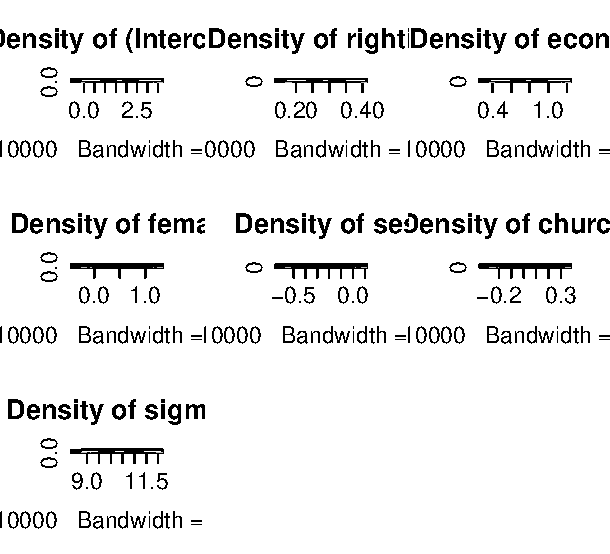
\includegraphics[width=\textwidth]{PS3-Figure1.pdf}
  \end{center}
  \caption{Density of Independent Variable}
  \label{f:f1}
\end{figure}

As we can see in the section 2 of the summary, the 95\% confidence interval of righttide ideology falls between 0.2370 and 0.34258 (both larger than 0). Thus we conclude that it is statistically significant that righttide ideology has a 0.28961 coefficient effect on people's preference to PRI: with one unit increase in righttide leaning, the person's preference to PRI increases by 0.28961 (section 1).



\item Suppose the literature further suggests that the effect of ideology on respondents' feelings about the PRI would be weaker among those who held more positive assessments of the national economy's recent performance.  Assess this conditional hypothesis using Empirical Bayes and the other default settings of MCMCpack.  \\

\begin{Schunk}
\begin{Sinput}
> m2<-MCMCregress(PRIfeel~rightide+econnat+rightide:econnat+female+ses+churchatt,data=mex,burnin = 1000, mcmc = 10000,
+     thin = 1, verbose = 0, seed = 19880201, beta.start = NA, 
+     b0 = 0, B0 = 0, c0 = 0.001, d0 = 0.001, sigma.mu = NA, sigma.var = NA, 
+     marginal.likelihood =("none") )
> summary(m2)
\end{Sinput}
\begin{Soutput}
Iterations = 1001:11000
Thinning interval = 1 
Number of chains = 1 
Sample size per chain = 10000 

1. Empirical mean and standard deviation for each variable,
   plus standard error of the mean:

                     Mean      SD  Naive SE Time-series SE
(Intercept)       1.41214 0.62440 0.0062440      0.0062440
rightide          0.33330 0.08212 0.0008212      0.0008076
econnat           0.89115 0.20099 0.0020099      0.0020099
female            0.53641 0.16154 0.0016154      0.0015916
ses              -0.23862 0.07374 0.0007374      0.0007374
churchatt         0.03804 0.07145 0.0007145      0.0007279
rightide:econnat -0.01598 0.02851 0.0002851      0.0002851
sigma2           10.39155 0.36606 0.0036606      0.0035053

2. Quantiles for each variable:

                     2.5%       25%      50%       75%    97.5%
(Intercept)       0.17666  0.988293  1.41492  1.832663  2.63241
rightide          0.16944  0.278760  0.33312  0.389432  0.49443
econnat           0.49626  0.755669  0.89095  1.028299  1.28377
female            0.21728  0.427948  0.53707  0.645899  0.85682
ses              -0.38200 -0.288061 -0.23851 -0.189034 -0.09362
churchatt        -0.10125 -0.009644  0.03751  0.086170  0.17828
rightide:econnat -0.07107 -0.035582 -0.01618  0.003339  0.04018
sigma2            9.69708 10.137559 10.37946 10.629708 11.13262
\end{Soutput}
\end{Schunk}

\begin{Schunk}
\begin{Sinput}
> # library(stargazer)
> # stargazer(m1,m2,title="MCMC regression Results",
> #          dep.var.labels="Feeling about the PRI",
> #          covariate.labels=c("Ideology", "National Economy", "Female", "SES", "Church Attend."),
> #          align=TRUE, 
> #          omit.stat=c("adj.rsq","f","ser"),
> #          label="T:res"
> #          )
\end{Sinput}
\end{Schunk}

According to m2, the effect of postivive national economy assessment on righttide respondents'' feeling about the PRI is sum of the coefficient of econnat and the coefficient of interaction term. As we can see from the section 1 of the output, "econnat (beta3)=0.89115" and "rightide:econnat(beta7)= -0.01598", the influence of positive economy performance on preference to PRI is 0.89115+(-0.01598). Since the coefficient of rightide:econnat is negative, it means the positive assessments of the national economy weakens the effect of ideology  on feeling about the PRI. Thus the result does support the conditional hypothesis. 

\item Suppose a ``helpful'' reviewer points out that Empirical Bayes imposes a very strong set of priors, and that noninformative priors may yield a different result.  Going well beyond the call of duty, this reviewer even offers some code for you to study and then try out.  Is the reviewer correct that your conclusions regarding the conditional hypothesis change with a different prior?  \\

\begin{Schunk}
\begin{Sinput}
> require(rstan)
> # First we have to define the model
> PRIfeel.code <- '
+     data {
+         int<lower=0> N;
+         vector[N] PRIfeel;
+         vector[N] rightide;
+         vector[N] econnat;
+         vector[N] female;
+         vector[N] ses;
+         vector[N] churchatt;
+     }
+     transformed data {
+         vector[N] rightideXeconnat;
+         rightideXeconnat <- rightide .* econnat;
+     }
+     parameters {                
+         real beta1;             // coef for constant (default prior is uniform, i.e., noninformative)
+         real beta2;             
+         real beta3;
+         real beta4;
+         real beta5;
+         real beta6;
+         real beta7;
+         real<lower=0> sigma;
+     }
+     model {
+         PRIfeel ~ normal(beta1 + beta2 * rightide + beta3 * econnat +
+                              beta4 * female + beta5 * ses +
+                              beta6 * churchatt + beta7 * rightideXeconnat, sigma);
+     }
+ '
> # Then put the data into the expected format
> mex.data <- list(N = nrow(mex), PRIfeel = mex$PRIfeel, rightide = mex$rightide,
+                    econnat = mex$econnat, female = mex$female, 
+                    ses = mex$ses, churchatt = mex$churchatt)
> # Now we can run it
> set.seed(324)
> m2.stan <- stan(model_code = PRIfeel.code, data = mex.data, 
+                 iter = 1000, chains = 3)
\end{Sinput}
\begin{Soutput}
TRANSLATING MODEL 'PRIfeel.code' FROM Stan CODE TO C++ CODE NOW.
COMPILING THE C++ CODE FOR MODEL 'PRIfeel.code' NOW.
cygwin warning:
  MS-DOS style path detected: C:/PROGRA~1/R/R-30~1.2/etc/x64/Makeconf
  Preferred POSIX equivalent is: /cygdrive/c/PROGRA~1/R/R-30~1.2/etc/x64/Makeconf
  CYGWIN environment variable option "nodosfilewarning" turns off this warning.
  Consult the user's guide for more details about POSIX paths:
    http://cygwin.com/cygwin-ug-net/using.html#using-pathnames
C:/Users/kellengracey/Documents/R/win-library/3.0/rstan/include//stansrc/stan/agrad/rev/var_stack.hpp:49:17: warning: 'void stan::agrad::free_memory()' defined but not used [-Wunused-function]
C:/Users/kellengracey/Documents/R/win-library/3.0/rstan/include//stansrc/stan/agrad/rev/chainable.hpp:87:17: warning: 'void stan::agrad::set_zero_all_adjoints()' defined but not used [-Wunused-function]
SAMPLING FOR MODEL 'PRIfeel.code' NOW (CHAIN 1).

Iteration:   1 / 1000 [  0%]  (Warmup)
Iteration: 100 / 1000 [ 10%]  (Warmup)
Iteration: 200 / 1000 [ 20%]  (Warmup)
Iteration: 300 / 1000 [ 30%]  (Warmup)
Iteration: 400 / 1000 [ 40%]  (Warmup)
Iteration: 500 / 1000 [ 50%]  (Warmup)
Iteration: 600 / 1000 [ 60%]  (Sampling)
Iteration: 700 / 1000 [ 70%]  (Sampling)
Iteration: 800 / 1000 [ 80%]  (Sampling)
Iteration: 900 / 1000 [ 90%]  (Sampling)
Iteration: 1000 / 1000 [100%]  (Sampling)
Elapsed Time: 19.033 seconds (Warm-up)
              15.515 seconds (Sampling)
              34.548 seconds (Total)

SAMPLING FOR MODEL 'PRIfeel.code' NOW (CHAIN 2).

Iteration:   1 / 1000 [  0%]  (Warmup)
Iteration: 100 / 1000 [ 10%]  (Warmup)
Iteration: 200 / 1000 [ 20%]  (Warmup)
Iteration: 300 / 1000 [ 30%]  (Warmup)
Iteration: 400 / 1000 [ 40%]  (Warmup)
Iteration: 500 / 1000 [ 50%]  (Warmup)
Iteration: 600 / 1000 [ 60%]  (Sampling)
Iteration: 700 / 1000 [ 70%]  (Sampling)
Iteration: 800 / 1000 [ 80%]  (Sampling)
Iteration: 900 / 1000 [ 90%]  (Sampling)
Iteration: 1000 / 1000 [100%]  (Sampling)
Elapsed Time: 16.467 seconds (Warm-up)
              13.32 seconds (Sampling)
              29.787 seconds (Total)

SAMPLING FOR MODEL 'PRIfeel.code' NOW (CHAIN 3).

Iteration:   1 / 1000 [  0%]  (Warmup)
Iteration: 100 / 1000 [ 10%]  (Warmup)
Iteration: 200 / 1000 [ 20%]  (Warmup)
Iteration: 300 / 1000 [ 30%]  (Warmup)
Iteration: 400 / 1000 [ 40%]  (Warmup)
Iteration: 500 / 1000 [ 50%]  (Warmup)
Iteration: 600 / 1000 [ 60%]  (Sampling)
Iteration: 700 / 1000 [ 70%]  (Sampling)
Iteration: 800 / 1000 [ 80%]  (Sampling)
Iteration: 900 / 1000 [ 90%]  (Sampling)
Iteration: 1000 / 1000 [100%]  (Sampling)
Elapsed Time: 18.818 seconds (Warm-up)
              13.382 seconds (Sampling)
              32.2 seconds (Total)
\end{Soutput}
\begin{Sinput}
> print(m2.stan)
\end{Sinput}
\begin{Soutput}
Inference for Stan model: PRIfeel.code.
3 chains, each with iter=1000; warmup=500; thin=1; 
post-warmup draws per chain=500, total post-warmup draws=1500.

         mean se_mean  sd    2.5%     25%     50%     75%   97.5% n_eff Rhat
beta1     1.5     0.0 0.6     0.3     1.0     1.4     1.9     2.7   472    1
beta2     0.3     0.0 0.1     0.2     0.3     0.3     0.4     0.5   522    1
beta3     0.9     0.0 0.2     0.5     0.7     0.9     1.0     1.3   552    1
beta4     0.5     0.0 0.2     0.2     0.4     0.5     0.6     0.8  1143    1
beta5    -0.2     0.0 0.1    -0.4    -0.3    -0.2    -0.2    -0.1   924    1
beta6     0.0     0.0 0.1    -0.1     0.0     0.0     0.1     0.2   968    1
beta7     0.0     0.0 0.0    -0.1     0.0     0.0     0.0     0.0   523    1
sigma     3.2     0.0 0.1     3.1     3.2     3.2     3.3     3.3  1155    1
lp__  -2713.0     0.1 2.0 -2717.6 -2714.1 -2712.7 -2711.6 -2710.2   562    1

Samples were drawn using NUTS(diag_e) at Thu Mar 13 10:03:10 2014.
For each parameter, n_eff is a crude measure of effective sample size,
and Rhat is the potential scale reduction factor on split chains (at 
convergence, Rhat=1).
\end{Soutput}
\begin{Sinput}
> m2.stan.sim <- as.data.frame(m2.stan)
> 
> 
> 
\end{Sinput}
\end{Schunk}

As we can see from the output, beta2=0.3 (MCMC rightide:0.333), beta3=0.9 (MCMC econnat:0.891), beta4=0.5 (MCMC female=0.536), beta5=-0.2 (MCMC ses=-0.239),beta6=0.0 (MCMC churchatt=0.038), beta7=0.0 (MCMC rightide:econnat=-0.016), the stan result with weak priors (uniform distribution) do not yield a very different result.

            b          lb          ub
1  1.45680481  0.20047082  2.65509789
2  0.32983824  0.16562228  0.49026322
3  0.88123471  0.49915704  1.28159359
4  0.52589903  0.20198199  0.83908045
5 -0.24496189 -0.38062972 -0.10160730
6  0.04090839 -0.09469561  0.19153111
7 -0.01489438 -0.07351261  0.04247551
\item Assess the original, unconditional hypothesis using noninformative priors.  Include a graph of the posterior distribution for the effect of ideology on feelings toward the PRI.  Also graph the highest density intervals of the posteriors of the effects of all variables in the model, remembering to standardize the continuous variables by dividing them by twice their standard deviations. 

\begin{Schunk}
\begin{Sinput}
> # First define the model for the original, unconditional hypothesis
> PRIfeel.code.1 <- '
+     data {
+         int<lower=0> N;
+         vector[N] PRIfeel;
+         vector[N] rightide;
+         vector[N] econnat;
+         vector[N] female;
+         vector[N] ses;
+         vector[N] churchatt;
+     }
+    
+     parameters {                
+         real beta1;             // coef for constant (default prior is uniform, i.e., noninformative)
+         real beta2;             
+         real beta3;
+         real beta4;
+         real beta5;
+         real beta6;
+         real beta7;
+         real<lower=0> sigma;
+     }
+     model {
+         PRIfeel ~ normal(beta1 + beta2 * rightide + beta3 * econnat +
+                              beta4 * female + beta5 * ses +
+                              beta6 * churchatt, sigma);
+     }
+ '
> # Then put the data into the expected format
> mex.data <- list(N = nrow(mex), PRIfeel = mex$PRIfeel, rightide = mex$rightide,
+                    econnat = mex$econnat, female = mex$female, 
+                    ses = mex$ses, churchatt = mex$churchatt)
> #run it
> set.seed(740)
> m1.stan <- stan(model_code = PRIfeel.code.1, data = mex.data, 
+                 iter = 1000, chains = 3)
\end{Sinput}
\begin{Soutput}
TRANSLATING MODEL 'PRIfeel.code.1' FROM Stan CODE TO C++ CODE NOW.
COMPILING THE C++ CODE FOR MODEL 'PRIfeel.code.1' NOW.
cygwin warning:
  MS-DOS style path detected: C:/PROGRA~1/R/R-30~1.2/etc/x64/Makeconf
  Preferred POSIX equivalent is: /cygdrive/c/PROGRA~1/R/R-30~1.2/etc/x64/Makeconf
  CYGWIN environment variable option "nodosfilewarning" turns off this warning.
  Consult the user's guide for more details about POSIX paths:
    http://cygwin.com/cygwin-ug-net/using.html#using-pathnames
C:/Users/kellengracey/Documents/R/win-library/3.0/rstan/include//stansrc/stan/agrad/rev/var_stack.hpp:49:17: warning: 'void stan::agrad::free_memory()' defined but not used [-Wunused-function]
C:/Users/kellengracey/Documents/R/win-library/3.0/rstan/include//stansrc/stan/agrad/rev/chainable.hpp:87:17: warning: 'void stan::agrad::set_zero_all_adjoints()' defined but not used [-Wunused-function]
SAMPLING FOR MODEL 'PRIfeel.code.1' NOW (CHAIN 1).

Iteration:   1 / 1000 [  0%]  (Warmup)
Iteration: 100 / 1000 [ 10%]  (Warmup)
Iteration: 200 / 1000 [ 20%]  (Warmup)
Iteration: 300 / 1000 [ 30%]  (Warmup)
Iteration: 400 / 1000 [ 40%]  (Warmup)
Iteration: 500 / 1000 [ 50%]  (Warmup)
Iteration: 600 / 1000 [ 60%]  (Sampling)
Iteration: 700 / 1000 [ 70%]  (Sampling)
Iteration: 800 / 1000 [ 80%]  (Sampling)
Iteration: 900 / 1000 [ 90%]  (Sampling)
Iteration: 1000 / 1000 [100%]  (Sampling)
Elapsed Time: 65.718 seconds (Warm-up)
              56.289 seconds (Sampling)
              122.007 seconds (Total)

SAMPLING FOR MODEL 'PRIfeel.code.1' NOW (CHAIN 2).

Iteration:   1 / 1000 [  0%]  (Warmup)
Iteration: 100 / 1000 [ 10%]  (Warmup)
Iteration: 200 / 1000 [ 20%]  (Warmup)
Iteration: 300 / 1000 [ 30%]  (Warmup)
Iteration: 400 / 1000 [ 40%]  (Warmup)
Iteration: 500 / 1000 [ 50%]  (Warmup)
Iteration: 600 / 1000 [ 60%]  (Sampling)
Iteration: 700 / 1000 [ 70%]  (Sampling)
Iteration: 800 / 1000 [ 80%]  (Sampling)
Iteration: 900 / 1000 [ 90%]  (Sampling)
Iteration: 1000 / 1000 [100%]  (Sampling)
Elapsed Time: 60.727 seconds (Warm-up)
              51.198 seconds (Sampling)
              111.925 seconds (Total)

SAMPLING FOR MODEL 'PRIfeel.code.1' NOW (CHAIN 3).

Iteration:   1 / 1000 [  0%]  (Warmup)
Iteration: 100 / 1000 [ 10%]  (Warmup)
Iteration: 200 / 1000 [ 20%]  (Warmup)
Iteration: 300 / 1000 [ 30%]  (Warmup)
Iteration: 400 / 1000 [ 40%]  (Warmup)
Iteration: 500 / 1000 [ 50%]  (Warmup)
Iteration: 600 / 1000 [ 60%]  (Sampling)
Iteration: 700 / 1000 [ 70%]  (Sampling)
Iteration: 800 / 1000 [ 80%]  (Sampling)
Iteration: 900 / 1000 [ 90%]  (Sampling)
Iteration: 1000 / 1000 [100%]  (Sampling)
Elapsed Time: 51.59 seconds (Warm-up)
              64.353 seconds (Sampling)
              115.943 seconds (Total)
\end{Soutput}
\begin{Sinput}
> print(m1.stan)
\end{Sinput}
\begin{Soutput}
Inference for Stan model: PRIfeel.code.1.
3 chains, each with iter=1000; warmup=500; thin=1; 
post-warmup draws per chain=500, total post-warmup draws=1500.

               mean      se_mean           sd          2.5%           25%
beta1  1.700000e+00 0.000000e+00 4.000000e-01  9.000000e-01  1.400000e+00
beta2  3.000000e-01 0.000000e+00 0.000000e+00  2.000000e-01  3.000000e-01
beta3  8.000000e-01 0.000000e+00 1.000000e-01  6.000000e-01  7.000000e-01
beta4  5.000000e-01 0.000000e+00 2.000000e-01  2.000000e-01  4.000000e-01
beta5 -2.000000e-01 0.000000e+00 1.000000e-01 -4.000000e-01 -3.000000e-01
beta6  0.000000e+00 0.000000e+00 1.000000e-01 -1.000000e-01  0.000000e+00
beta7 -3.067249e+10 7.188182e+10 2.043065e+11 -5.281614e+11 -1.497746e+11
sigma  3.200000e+00 0.000000e+00 1.000000e-01  3.100000e+00  3.200000e+00
lp__  -2.712700e+03 1.000000e-01 1.900000e+00 -2.717700e+03 -2.713800e+03
                50%           75%         97.5% n_eff Rhat
beta1  1.700000e+00           2.0  2.500000e+00  1136  1.0
beta2  3.000000e-01           0.3  3.000000e-01  1500  1.0
beta3  8.000000e-01           0.9  1.000000e+00  1500  1.0
beta4  5.000000e-01           0.7  9.000000e-01  1500  1.0
beta5 -2.000000e-01          -0.2 -1.000000e-01  1408  1.0
beta6  0.000000e+00           0.1  2.000000e-01  1500  1.0
beta7 -5.381888e+10 82099682387.2  3.436403e+11     8  1.6
sigma  3.200000e+00           3.3  3.300000e+00  1500  1.0
lp__  -2.712400e+03       -2711.3 -2.710000e+03   633  1.0

Samples were drawn using NUTS(diag_e) at Thu Mar 13 10:09:31 2014.
For each parameter, n_eff is a crude measure of effective sample size,
and Rhat is the potential scale reduction factor on split chains (at 
convergence, Rhat=1).
\end{Soutput}
\begin{Sinput}
> m1.stan.sim <- as.data.frame(m1.stan)
\end{Sinput}
\end{Schunk}

As we can see in the output of stan model m1 (as well as Figure 2), the 95\% confidence interval of righttide ideology falls between 0.2 and 0.3 (both larger than 0). Thus we conclude that it is statistically significant that righttide ideology has a 0.3 coefficient effect on people's preference to PRI: with one unit increase in righttide leaning, the person's preference to PRI increases by 0.3.



\begin{Schunk}
\begin{Soutput}
SAMPLING FOR MODEL 'PRIfeel.code.1' NOW (CHAIN 1).

Iteration:   1 / 1000 [  0%]  (Warmup)
Iteration: 100 / 1000 [ 10%]  (Warmup)
Iteration: 200 / 1000 [ 20%]  (Warmup)
Iteration: 300 / 1000 [ 30%]  (Warmup)
Iteration: 400 / 1000 [ 40%]  (Warmup)
Iteration: 500 / 1000 [ 50%]  (Warmup)
Iteration: 600 / 1000 [ 60%]  (Sampling)
Iteration: 700 / 1000 [ 70%]  (Sampling)
Iteration: 800 / 1000 [ 80%]  (Sampling)
Iteration: 900 / 1000 [ 90%]  (Sampling)
Iteration: 1000 / 1000 [100%]  (Sampling)
Elapsed Time: 62.964 seconds (Warm-up)
              59.3 seconds (Sampling)
              122.264 seconds (Total)

SAMPLING FOR MODEL 'PRIfeel.code.1' NOW (CHAIN 2).

Iteration:   1 / 1000 [  0%]  (Warmup)
Iteration: 100 / 1000 [ 10%]  (Warmup)
Iteration: 200 / 1000 [ 20%]  (Warmup)
Iteration: 300 / 1000 [ 30%]  (Warmup)
Iteration: 400 / 1000 [ 40%]  (Warmup)
Iteration: 500 / 1000 [ 50%]  (Warmup)
Iteration: 600 / 1000 [ 60%]  (Sampling)
Iteration: 700 / 1000 [ 70%]  (Sampling)
Iteration: 800 / 1000 [ 80%]  (Sampling)
Iteration: 900 / 1000 [ 90%]  (Sampling)
Iteration: 1000 / 1000 [100%]  (Sampling)
Elapsed Time: 61.037 seconds (Warm-up)
              60.491 seconds (Sampling)
              121.528 seconds (Total)

SAMPLING FOR MODEL 'PRIfeel.code.1' NOW (CHAIN 3).

Iteration:   1 / 1000 [  0%]  (Warmup)
Iteration: 100 / 1000 [ 10%]  (Warmup)
Iteration: 200 / 1000 [ 20%]  (Warmup)
Iteration: 300 / 1000 [ 30%]  (Warmup)
Iteration: 400 / 1000 [ 40%]  (Warmup)
Iteration: 500 / 1000 [ 50%]  (Warmup)
Iteration: 600 / 1000 [ 60%]  (Sampling)
Iteration: 700 / 1000 [ 70%]  (Sampling)
Iteration: 800 / 1000 [ 80%]  (Sampling)
Iteration: 900 / 1000 [ 90%]  (Sampling)
Iteration: 1000 / 1000 [100%]  (Sampling)
Elapsed Time: 62.597 seconds (Warm-up)
              67 seconds (Sampling)
              129.597 seconds (Total)
\end{Soutput}
\begin{Soutput}
              b            lb            ub
1  1.674333e+00  8.322711e-01  2.465160e+00
2  2.895542e-01  2.397764e-01  3.422557e-01
3  7.922801e-01  6.111619e-01  9.722532e-01
4  5.454781e-01  2.174920e-01  8.527266e-01
5 -2.385065e-01 -3.676629e-01 -8.157804e-02
6  3.693938e-02 -1.148660e-01  1.671959e-01
7 -3.067249e+10 -3.287967e+11  3.924809e+11
\end{Soutput}
\end{Schunk}

\begin{figure}[htbp] 
  \caption{Posterior Distribution of the Effect of Ideology}
  \label{F:postide}
  \begin{center}
    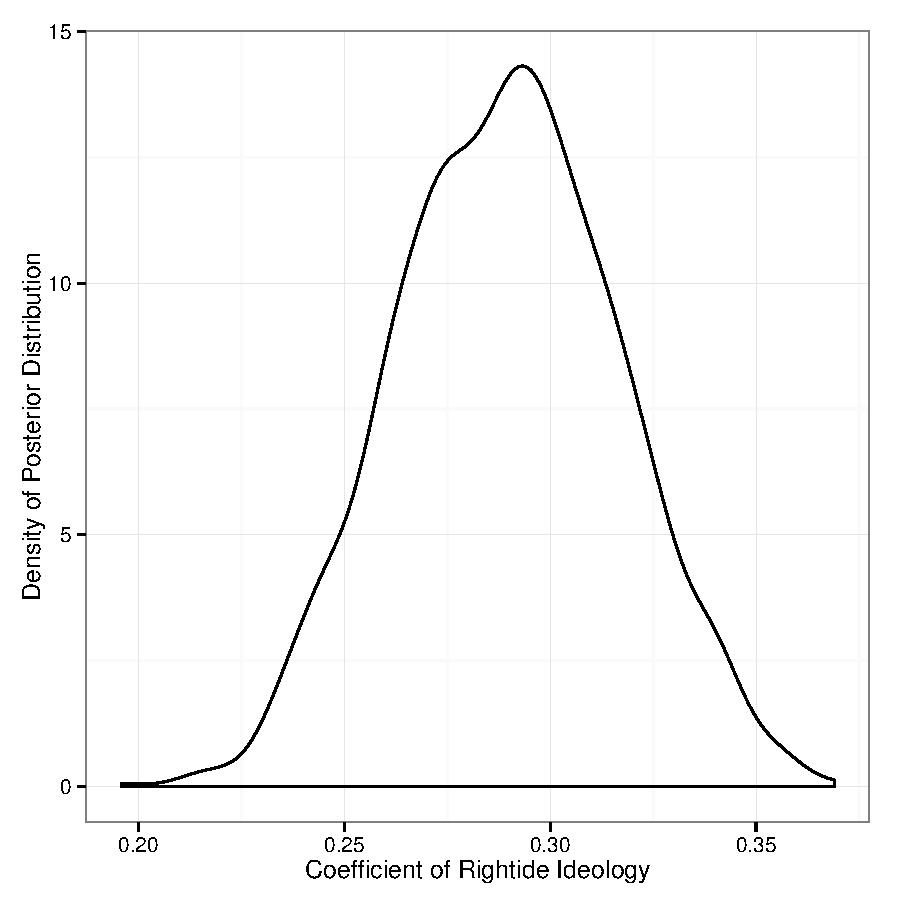
\includegraphics[width=5.25in]{PS3-f1.pdf}
  \end{center}
\end{figure}

\begin{figure}[htbp] 
  \caption{Posterior Distribution of the Effect of Ideology}
  \label{F:postide}
  \begin{center}
    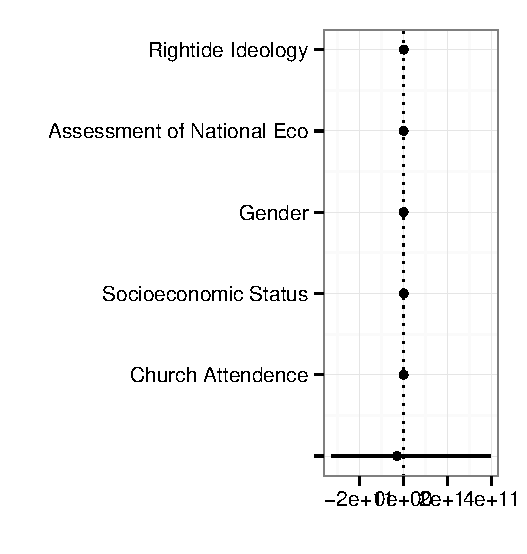
\includegraphics[width=5.25in]{PS3-f2.pdf}
  \end{center}
  \begin{footnotesize}
  \begin{tabular}{p{.4in} p{4.75in}}
  & \emph{Note}: Continuous variables rescaled by dividing by twice their standard deviations per \citet{Gelman2008}.
  \end{tabular}
  \end{footnotesize}
\end{figure}


\bibliographystyle{ajps}
\bibliography{PS3Library}

\end{enumerate}
\end{document}
=======
+     marginal.likelihood =("none") )
>>>>>>> 7aa62a21968e215f5350ff120fc5a09736db651c
